\chapter{Large Language Models}
\label{cap:large_language_models}

% TODO:daniel: Hacer capítulo de Large Language Models

\section{Historia de los Large Language Models}
\label{sec:historia}

El lenguaje es una de las habilidades más importantes que tenemos los seres humanos, y es
que gracias a esta habilidad podemos comunicarnos entre nosotros. Pero, las maquinas no
tienen esta habilidad, a menos que las equipemos on algoritmos poderosos de inteligencia
artificial. Pero aun así siempre a sido un reto conseguir que las maquinas puedan leer, 
escribir y comunicarse como los humanos.

\begin{figure}[H]
    \begin{center}
      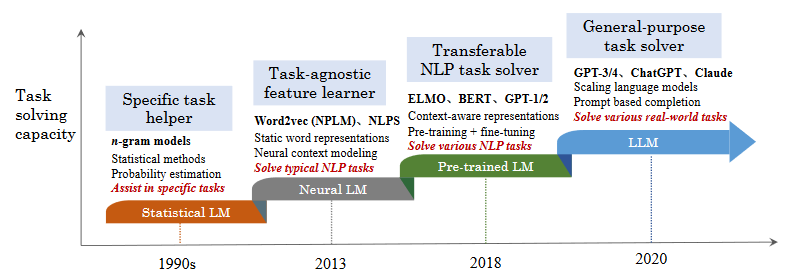
\includegraphics[width=15cm]{figuras/Capitulo_09/EvolutionLM.png}
    \end{center}
    \caption[Proceso de evolución de las cuatro generaciones de modelos lingüísticos (LM) desde la perspectiva de la capacidad de resolución de tareas.]{Proceso de evolución de las cuatro generaciones de modelos lingüísticos (LM) desde la perspectiva de la capacidad de resolución de tareas.(\cite{ZhaoWayneXin2023ASoL})}
    \label{fig:evolutionLM}
\end{figure}\

\textit{Lenguage modeling} (LM) es, a dia de hoy, una de las mejores aproximaciones para conseguir
que las maquinas puedan entender el lenguage humano. La investigación en LM se puede dividir
en cuatro etapas \cite{ZhaoWayneXin2023ASoL}:

% TODO:daniel: Revisar la traducción de este párrafo

\begin{enumerate}
    \item \textit{\textbf{Statistical language models (SLM)}}: Estos modelos estan desarrollados basados en aprendizaje
        estadiístico, y se basan en la probabilidad de que una secuencia de palabras aparezca en un texto. Los 
        SLM se ha aplicado ampliamente para mejorar el rendimeitno de las tareas de recuperación de información
        y el procesamiento del lenguaje natural. Sin embargo, los SLM tienen una gran limitación, es díficil
        estimar con precisión modelos lingüísticos de alto orden exponencial de probabilidades de transición.
    \item \textit{\textbf{Neural language models (NLM)}}: Los NLM se basan en redes neuronales para estimar la probabilidad
        de una secuencia de palabras. Los NLM han demostrado ser más efectivos que los SLM, pero tienen una gran
        limitación, y es que se necesitan grandes cantidades de datos de entrenamiento para poder obtener buenos
        resultados.
    \item \textit{\textbf{Pre-trained language models (PLM)}}: Los PLM son modelos lingüísticos preentrenados que se pueden
        utilizar para resolver tareas de procesamiento de lenguaje natural. Los PLM se entrenan en grandes conjuntos
        de datos de texto sin etiquetar, y se pueden utilizar para resolver tareas de procesamiento de lenguaje
        natural (NLP) específicas con un ajuste fino. Los PLM han demostrado ser muy efectivos en una amplia gama
        de tareas de NLP, pero tienen una gran limitación, y es que se necesitan grandes cantidades de datos de
        entrenamiento para poder obtener buenos resultados.
    \item \textit{\textbf{Large language models (LLM)}}: Los LLM son modelos lingüísticos que se entrenan en grandes conjuntos
        de datos de texto sin etiquetar y se pueden utilizar para resolver tareas de NLP específicas con un ajuste
        fino. Los LLM han demostrado ser muy efectivos en una amplia gama de tareas de NLP, y se pueden entrenar
        con conjuntos de datos de entrenamiento más pequeños que los PLM.
\end{enumerate}

En mi caso, haremos incapie en los LLM, ya que son los modelos que se han utilizado para la realización de este
proyecto. Tipicamente los \textit{Large Language Models} se refiere a modelos de lenguajes que 
tienen cientos de billones de parámetros, y que son entrenados con datos masivos de texto.
Algunos de estos modelos son GPT-3, PaLM, Galactica o LLaMA. Estos modelos han demostrado altas
capacidades para entender el lenguaje natural y resolver tareas complejas a traves del lenguaje o texto.

Así mismo, dentro de los LLM estos han hido creciendo en tamaño y en cantidad de parámetros.
Para ilustralo, en la figura \ref{fig:evolutionLLM} podemos ver la evolución de los LLM a lo largo

\begin{figure}[H]
    \begin{center}
      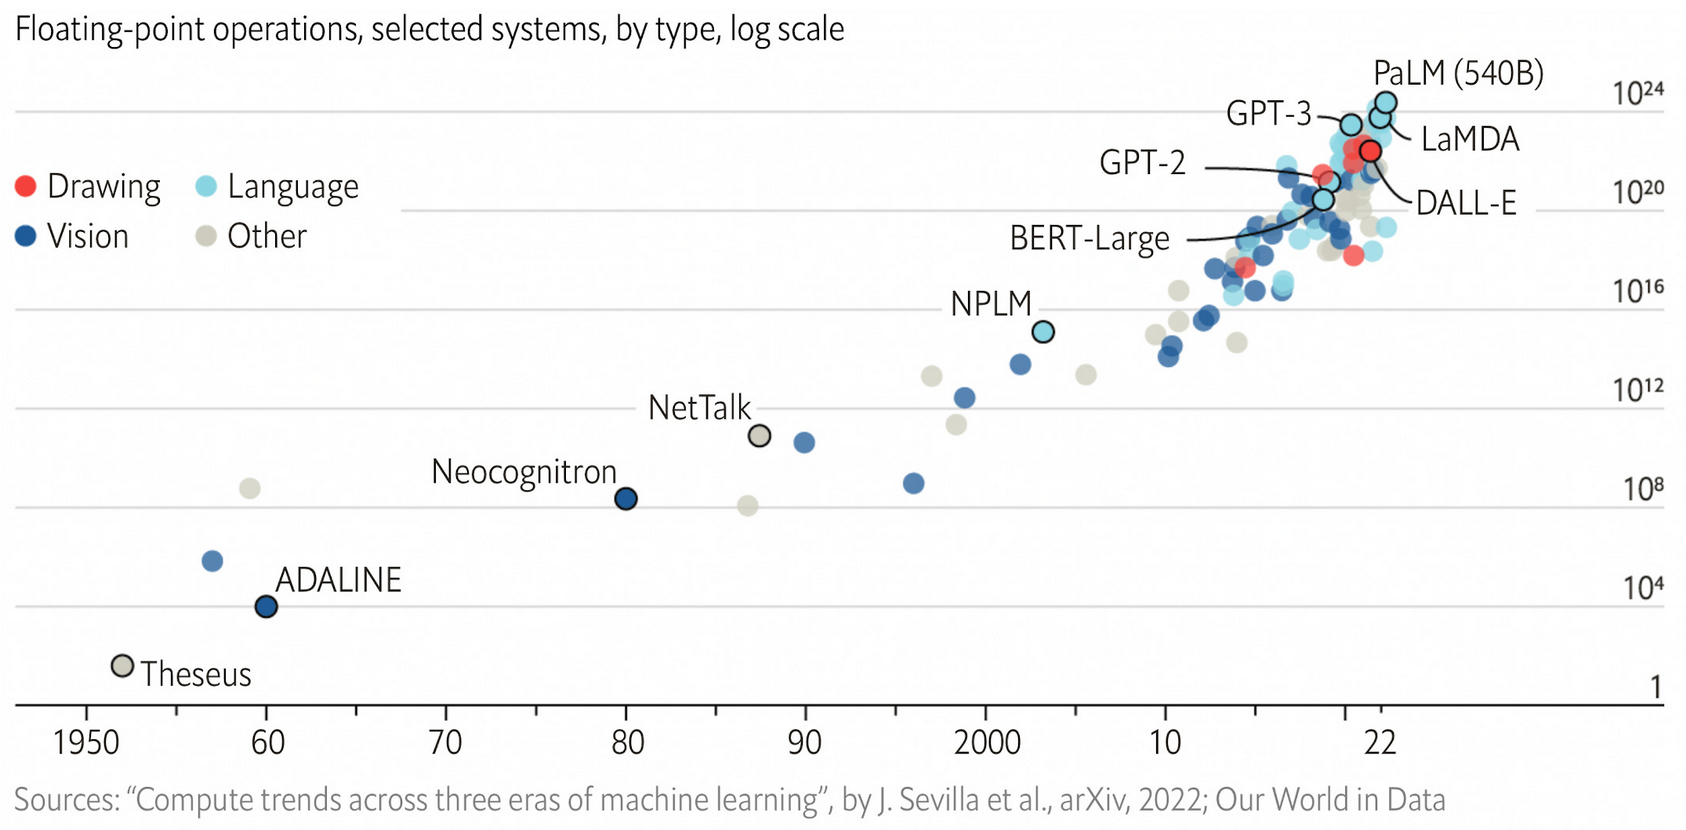
\includegraphics[width=15cm]{figuras/Capitulo_09/EvolutionLLM.png}
    \end{center}
    \caption[Operaciones de coma flotante por tipo en escala logarítmica]{Operaciones de coma flotante por tipo en escala logarítmica (\cite{EvolutionLLM})}
    \label{fig:evolutionLLM}
\end{figure}\

Pero lo que hace realmente interesante estos tipos de modelos es el concepto de
\textit{emergent abilities}, que nos viene a decir que hay abilidades que en 
modelos pequeños no se observan pero que en modelos grandes aparecen. Tres
habilidades que se han observado en los modelos grandes son:

\begin{itemize}
    \item \textbf{\textit{In-context learning}:} esta habilidad es la capacidad
        de generar el texto correcto a partir de una o mas instrucciones en texto
        natural mas un conjunto de demostraciones de como se debe realizar la tarea.
        El modelo es capaz de realizar la tarea sin necesidad de entrenamiento previo.
        Esta habilidad fue introducida formalmente por GPT-3.
    \item \textbf{\textit{Instruction following}:} esta es la habilidad de seguir
        instrucciones por las cuales no se a entrenado, es decir, si hacemos un 
        \textit{fine-tuning} de un modelo con un conjunto de multitareas formateadas en
        lenguaje natural, el modelo es capaz de realizar las tareas sin necesidad de
        entrenamiento previo.
    \item \textbf{\textit{Step-by-Step reasoning}:} esta es la habilidad de resolver
        problemas de razonamiento complejos, concretamente en resolver tareas que
        requieren de multiples pasos de razonamiento.
\end{itemize}

\section{Fine-tuning}
\label{sec:fine_tuning}

\begin{wrapfigure}{r}{0.3\textwidth}
    \centering
    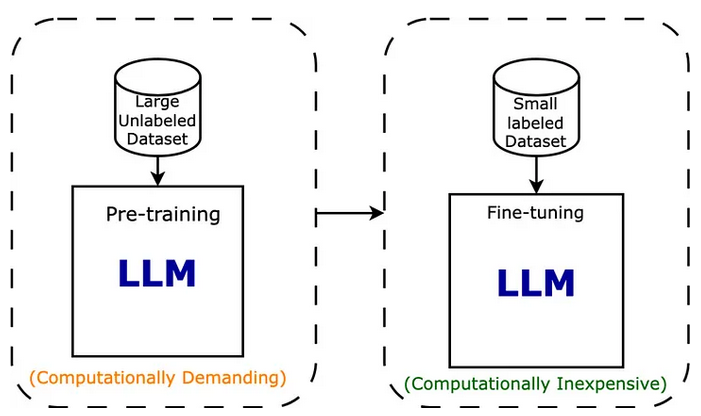
\includegraphics[width=0.3\textwidth]{figuras/Capitulo_09/TrainVSFinetuning.png}
    \caption[Entrenamiento versus \textit{fine-tuning}]{Entrenamiento versus \textit{fine-tuning} (\cite{SupervisedFineTuning})}
    \label{fig:finetuningVStraining}
\end{wrapfigure}

El \textit{fine-tuning} o en castellano ''ajuste fino'' es una técnica en la cual podemos ajustar 
ciertos pesos en las capas de nuestra red neuronal, de tal manera que podamos afinar los
resultados de nuestro modelo para una tarea en específico. Esta técnica se parte de un
modelo preentrenado y se van ajustando las diferenetes capas, en su totalidad o parcialmente,
con un conjunto de datos etiquetados. Esta técnica nos permite poder entrenar o ajustar los
modelos de manera eficiente y reduciendo los recursos computancionales y de memoria, pudiendo
incluso entrenar estos modelos en hardware de bajo coste o dispositivos comerciales para 
uso domestico.

Como he mencionado en la sección \ref{sec:historia}, los LLM tiene habilidades emergentes
que permiten que estos modelos puedan realizar tareas sin necesidad de entrenamiento previo.
Por lo tanto, en el \textit{fine-tuning} no buscamos enseñar al modelo como realizar una tarea si no 
mejorar la capacidad de realizar dicha tarea. \cite{Finetuning}

\begin{figure}[H]
    \begin{center}
      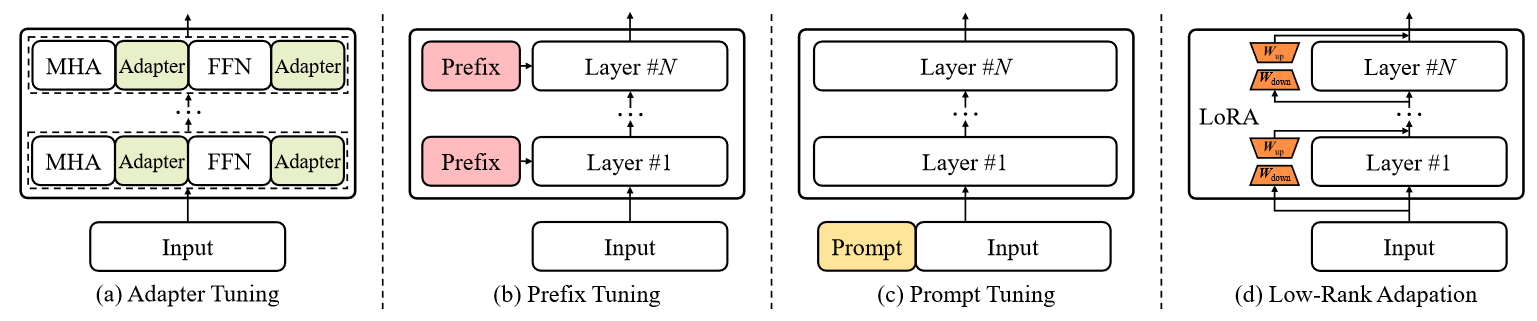
\includegraphics[width=15cm]{figuras/Capitulo_09/Finetuning.png}
    \end{center}
    \caption[]{(\cite{Finetuning})}
    \label{fig:finetuning}
\end{figure}\

Dentro de las tecnicas de \textit{fine-tuning} cabe destacar cinco metodos diferentes aunque en 
nuestro proyecto utilizaremos tan solo uno de ellos:

\begin{enumerate}
    \item \textit{\textbf{Prompt Tuning}}: El \textit{prompt tuning} es una técnica que consiste en
        añadir una pequeña cadena de texto al principio de la entrada, de tal manera que
        que con esta cadena ajustamos y ordenamos las intrucciones para nuestra tarea en
        especifico. Esta aproximación es la mas sencilla y rapida y que normalmente aplicamos
        cuando por ejemplo interactuamos con ChatGPT.
    \item \textit{\textbf{Prefix-tuning}}: El \textit{prefix-tuning} es una técnica que consiste en
        añadir una pequeña cadena de texto al principio de cada capa del modelo neuronal.
        Con esta capa lo que intentamos es ajustar y ordenar las instrucciones para nuestra
        tarea en especifico.
    \item \textit{\textbf{Adapter}}: este metodo incorpora modulos pequeños de redes neuronales,
        llamados adaptadores, que se conectan a las capas de salida de los modelos
        preentrenados. De tal manera que el proceso de \textit{fine-tuning} se optimizan los 
        adaptadores para la tarea en especifico mientras los del modelo original 
        quedan congelados. De esta manera se consigue reducir de manera considerable 
        el numero de parametros entrenables durante el \textit{fine-tuning}.
    \item \textit{\textbf{Low rank adaptation (Lora)}}: este metodo lo que hace es reducir el
        numero de parametros haciendo que la matriz de actualización sea de rango bajo.
        Consideremos una matriz de actualización $W$ y el proceso de \textit{fine-tuning}
        $W\leftarrow W + \bigtriangleup W$. LoRa propone congelar la matriz original
        $W\in \mathbb{R}^{m\times n}$ y convertir el proceso de actualización ($\bigtriangleup W$)
        bajando el rango de la matriz y descomponiendola, de tal manera que nos queda 
        $\bigtriangleup W = A\cdot B^T$ donde $A\in \mathbb{R}^{m\times k}$ y $B\in \mathbb{R}^{n\times k}$.
        \cite{ZhaoWayneXin2023ASoL}
    \item \textit{\textbf{QLoRa}}: este metodo reduce notablemente la cantidad de memoria 
        que se necesita para poder hacer el \textit{fine-tuning} de los modelos. Este metodo
        utiliza la técnica de \textit{LoRa} pero con una matriz de actualización cuantizada. De tal
        manera que la matriz de actualización se puede representar con un numero de bits
        mucho menor.\cite{DettmersTim2023QEFo}
\end{enumerate}

\begin{figure}[H]
    \begin{center}
      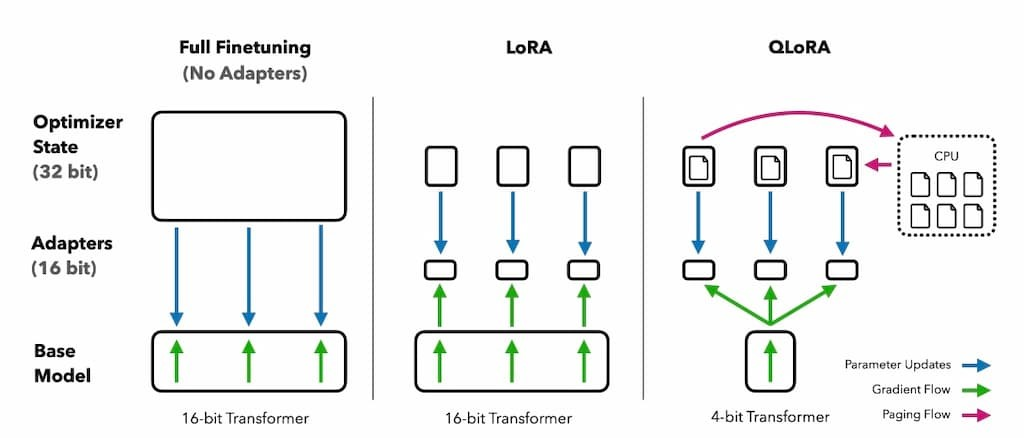
\includegraphics[width=13cm]{figuras/Capitulo_09/QLoRa.jpg}
    \end{center}
    \caption[]{(\cite{DettmersTim2023QEFo})}
    \label{fig:qlora}
\end{figure}\

% TODO:daniel: Mirar si podemos ampliar este capítulo con más información sobre los LLM

